\documentclass[class=article, crop=false]{standalone}
\usepackage{tikz}
\usepackage{subcaption}
\usetikzlibrary{calc}
\usetikzlibrary {shapes.geometric}

\begin{document}
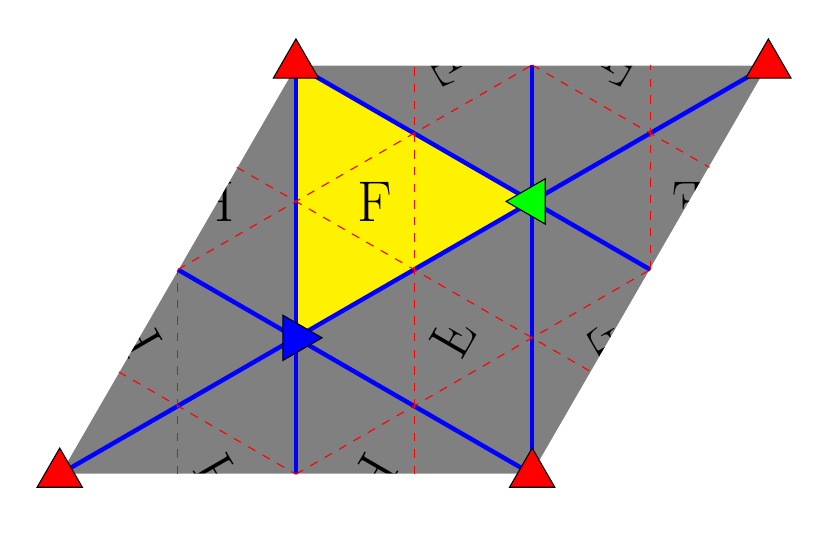
\begin{tikzpicture}
            % Define the lengths of the sides and the angle
            \def\a{3}  % length of side a
            \def\b{3}  % length of side b
            \def\angle{60}  % angle between sides a and b
            \def\s{F} % Label in center of cells

            \def\x{0.4}
            \def\y{0.4}
        
            % Calculate the coordinates of the points
            \coordinate (C00) at (0, 0);
            \coordinate (C10) at (\a, 0);
            \coordinate (C11) at ({\a + \b*cos(\angle)}, {\b * sin(\angle)});
            \coordinate (C01) at ({\b * cos(\angle)}, {\b * sin(\angle)});
            \coordinate (C02) at ({2*\b*cos(\angle)}, {2*\b * sin(\angle)});
            \coordinate (C12) at ({\a +2*\b * cos(\angle)}, {2*\b * sin(\angle)});
            \coordinate (C22) at ({2*\a + 2*\b * cos(\angle)}, {2*\b * sin(\angle)});
            \coordinate (C21) at ({2*\a + \b*cos(\angle)}, {\b * sin(\angle)});
            \coordinate (C20) at ({2*\a}, 0);
            \coordinate (A1) at ($(C00)!0.6666!(C11)$);
            \coordinate (A2) at ($(C11)!0.3333!(C22)$);
        

            % Draw the oblique unit cell
            \draw[thick,fill=gray,gray] (C00) -- (C20) -- (C22) -- (C02) -- cycle;
            \draw[thick,fill=yellow,yellow] (A1) -- (A2) -- (C02) -- cycle;
            %\draw[thick] (C10) -- (C21) -- (C12) -- (C01) -- cycle;
            

            % Draw bourdary chiral centres
            \node[rotate=240] at ($(C10)!0.3333!(C20)$) {\huge \s};
            \node[rotate=120] at ($(C00)!0.6666!(C10)$) {\reflectbox{\huge \s}};
            \node[rotate=120] at ($(C00)!0.6666!(C01)$) {\huge \s};
            \node at ($(C01)!0.3333!(C02)$) {\reflectbox{\huge \s}};
            \node[rotate=120] at ($(C02)!0.6666!(C12)$) {\reflectbox{\huge \s}};
            \node[rotate=240] at ($(C12)!0.3333!(C22)$) {\huge \s};
            \node[rotate=120] at ($(C20)!0.6666!(C21)$) {\huge \s};
            \node at ($(C21)!0.3333!(C22)$) {\reflectbox{\huge \s}};

            % Create white border
            \draw[fill=white,white] ($(C00)-(\x,\y)$) -- ($(C20)-(-\x,\y)$) -- (C20) -- (C00);
            \draw[fill=white,white] ($(C00)-(\x,-\y)$) -- ($(C02)-(\x,-\y)$) -- (C02) -- (C00);
            \draw[fill=white,white] ($(C02)+(\x,\y)$) -- ($(C22)-(\x,-\y)$) -- (C22) -- (C02);
            \draw[fill=white,white] ($(C20)+(\x,-\y)$) -- ($(C22)+(\x,\y)$) -- (C22) -- (C20);

            % Draw inner chiral centres
            \node at ($(A1)!0.5!(A2)!0.3333!(C02)$) {\huge \s};
            \node[rotate=240] at ($(A1)!0.5!(A2)!0.3333!(C20)$) {\reflectbox{\huge \s}};

        

            % Draw mirrow lines
            \draw[ultra thick,blue] (C00)--(C22);
            \draw[ultra thick,blue] (C01)--(C20);
            \draw[ultra thick,blue] (C10)--(C02);
            \draw[ultra thick,blue] (C12)--(C20);
            \draw[ultra thick,blue] (C02)--(C21);
            \draw[dashed,red] ($(C00)!0.5!(C10)$)--(C01);
            \draw[dashed,red] ($(C00)!0.5!(C01)$)--(C10);
            \draw[dashed,red] ($(C10)!0.5!(C20)$)--($(C02)!0.5!(C12)$);
            \draw[dashed,red] ($(C01)!0.5!(C02)$)--($(C20)!0.5!(C21)$);
            \draw[dashed,red] (C01)--(C12);
            \draw[dashed,red] (C10)--(C21);
            \draw[dashed,red] (C12)--($(C21)!0.5!(C22)$);
            \draw[dashed,red] (C21)--($(C12)!0.5!(C22)$);
            

            

            % Draw node reflections
            \draw (C00)  node[regular polygon, regular polygon sides=3, draw, fill=red, minimum size=0.5cm] {};
            %\draw (C10)  node[shape aspect=0.5,rotate=90,diamond,draw,fill=blue] {};
            %\draw (C11)  node[shape aspect=0.5,diamond,draw,fill=red] {};
            %\draw (C01)  node[shape aspect=0.5,rotate=90,diamond,draw,fill=blue] {};
            \draw (C02)  node[regular polygon, regular polygon sides=3, draw, fill=red, minimum size=0.5cm] {};
            %\draw (C12)  node[shape aspect=0.5,rotate=90,diamond,draw,fill=blue] {};
            \draw (C22)  node[regular polygon, regular polygon sides=3, draw, fill=red, minimum size=0.5cm] {};
            %\draw (C21)  node[shape aspect=0.5,rotate=90,diamond,draw,fill=blue] {};
            \draw (C20)  node[regular polygon, regular polygon sides=3, draw, fill=red, minimum size=0.5cm] {};

            \draw (A1)  node[rotate = 30,regular polygon, regular polygon sides=3, draw, fill=blue, minimum size=0.5cm] {};
            \draw (A2)  node[rotate=90, regular polygon, regular polygon sides=3, draw, fill=green, minimum size=0.5cm] {};

            %\draw ($(A)!0.5!(E)$) node[shape aspect=0.5,diamond,draw,fill=black] {};
            
        \end{tikzpicture}
\end{document}